\newpage
\section{Auswertung}
\label{sec:Auswertung}

\subsection{Bestimmung des vertikalen Erdmagnetfeldes}
\label{subsec:vertikal}

Es wurde im Versuch mithilfe eines Helmholtzspulenpaares ein vertikales Magnetfeld
erzeugt, das die vertikale Komponente des Erdmagnetfeldes kompensierte. Die vertikale
Komponente des Erdmagnetfeldes lässt sich daher aus den Daten des Helmholtzspulenpaares
mithilfe der Formel
\begin{equation}
    B= \mu_0 \cdot  \frac{8}{\sqrt {125}}\cdot \frac{I\cdot N}{R}
    \label{eqn:Helmholtz}
\end{equation}
berechnen. Mit den Daten aus der Versuchsanleitung \cite{Versuchsanleitung} und einem Strom von
$I_{vert}=0{,}195\,$A ergibt sich die vertikale Komponente des Erdmagnetfeldes zu
\begin{equation*}
  \SI{2.99e-5}{\tesla}\,.
\end{equation*}
Die Theoriewert hierzu ist (WERT + ZITAT).

\subsection{Bestimmung des horizontalen Erdmagnetfeldes und der Landé Faktoren}
\label{subsec:horizontal}

Zunächst werden mithilfe von Formel \eqref{eqn:Helmholtz} aus den gemessenen Stromstärken
die horizontalen Magnetfeldstärken berechnet. Die gemessenen und die daraus berechneten Werte befinden sich
in Tabelle \ref{tab:werte}.

\begin{table}[htp]
	\begin{center}
    \caption{Messwerte und daraus berechnete Werte für die magnetische Feldstärke.}
    \label{tab:werte}
		\begin{tabular}{ccccc}
		\toprule
			{$f$/kHz} & {$I_1$/A} & {$I_2$/A} & {$B_1$/µT} & {$B_2$/µT}\\
			\midrule
			100 & 0,42 & 0,50 & 25,35 & 30,17\\
			200 & 0,58 & 0,76 & 35,00 & 45,86\\
			300 & 0,76 & 1,00 & 45,86 & 60,35\\
			400 & 0,92 & 1,26 & 55,52 & 76,04\\
			500 & 1,09 & 1,51 & 65,78 & 91,12\\
			600 & 1,26 & 1,76 & 76,04 & 106,21\\
			700 & 1,43 & 2,01 & 86,30 & 121,30\\
			800 & 1,60 & 2,21 & 96,56 & 133,37\\
			900 & 1,76 & 2,52 & 106,21 & 152,08\\
			1000 & 1,93 & 2,77 & 116,47 & 167,16\\
		\bottomrule
		\end{tabular}
	\end{center}
\end{table}

Anschließend wird für beide Isotope getrennt jeweils die horizontale Magnetfeldstärke $B_hor$
gegen die Frequenz $f$ aufgetragen und es wird eine lineare Ausgleichsrechnung der Form
\begin{equation*}
  g(f)=af+b
\end{equation*}
durchgeführt. Es ergeben sich die Parameter
\begin{align*}
 a_1&= \SI{}{\tesla\per\Hz}  \,,\\
 b_1&= \SI{}{\tesla} \,,\\
 a_2&= \SI{}{\tesla\per\Hz} \,,\\
 b_2&= \SI{}{\tesla} \,.
\end{align*}
Die zugehörigen Plots sind in den Abbildungen \ref{fig:frequenz1} und \ref{fig:frequenz2} dargestellt.
\begin{figure}
  \centering
  \includegraphics[width=\textwidth]{build/frequenz1.pdf}
  \caption{Messwerte und Ausgleichsrechnung zur Bestimmung des horizontalen B-Feldes und des Landé-Faktors für
  das erste Isotop.}
  \label{fig:frequenz1}
\end{figure}
\begin{figure}
  \centering
  \includegraphics[width=\textwidth]{build/frequenz2.pdf}
  \caption{Messwerte und Ausgleichsrechnung zur Bestimmung des horizontalen B-Feldes und des Landé-Faktors für
  das zweite Isotop.}
  \label{fig:frequenz2}
\end{figure}
Aus den Parametern lassen sich nun die horizontale B-Feldstärke, sowie der Landé-Faktor bestimmen.
Die horizontale Erdmagnetfeldstärke ist gegeben durch den Parameter $b$. Der Theoriewerte beträgt hier
(WERT + ZITAT).

Der Landé-Faktor kann mithilfe von Formel \ref{eqn:B_M_Theorie} berechnet werden zu
\begin{equation*}
  g_F=\frac{4\pi m_e}{e a} \,.
\end{equation*}
Damit ergeben sich die beiden Werte
\begin{align*}
  g_{F,1}&= \,,\\
  g_{F,2}&= \,.
\end{align*}

\subsection{Bestimmung des Kernspins}
\label{subsec:Kernspin}

Für die beiden Rb Isotope gilt $L=0$, $S=\frac{1}{2}$ und $J=\frac{1}{2}$.
Es folgt für Formel \eqref{eqn:g_F_Theorie}
\begin{equation*}
  I=\frac{1}{2}\left(\frac{g_J}{g_F}-1\right) \,.
\end{equation*}
Der Landé-Faktor $g_J$ kann mithilfe von Formel \ref{eqn:g_J_Theorie} zu $g_J=2{,}0023$ bestimmt
werden. Für den Kernspin folgt damit
\begin{align*}
  I_1&= \,,\\
  I_2&= \,.
\end{align*}
Die Theoriewerte betragen hier $I=5/2$ für $\text{Rb}^{85}$ und $I=3/2$ für $\text{Rb}^{87}$.

Mithilfe des Kernspins können die Isotope wie folgt zugeordnet werden: Isotop 1 ist $\text{Rb}^{87}$
und Isotop 2 ist $\text{Rb}^{85}$.


\subsection{Bestimmung des Isotopenverhältnisses}
\label{subsec:Isotope}
In Abbildung \ref{fig:foto} ist ein typischer Verlauf der Transparenz des Rb-Gases in Abhängigkeit
von der magnetischen Feldstärke bei einer Frequenz von $f=100\,$kHz dargestellt.
Aus dem Verhältnis der Tiefen der Dips der beiden
Isotope lässt sich mithilfe von Formel \ref{eqn:transient} das Isotopenverhältnis bestimmen.
Für den ersten Dip ergibt sich eine Amplitude von 4{,}5 Einheiten und für den zweiten
eine Amplitude von 9 Einheiten
\begin{equation}
  \frac{\gamma_{85}}{\gamma_{87}}=\frac{9}{4{,}5}= 2 \,.
\end{equation}

Das in der Natur vorkommende Verhältnis folgt aus den Verhältnissen der beiden Isotope (ZITAT!!!)
und ergibt
\begin{equation}
  \frac{\text{Anteil}~ \ce{^{85}Rb}}{\text{Anteil}~ \ce{^{87}Rb}}=\frac{72,12\%}{27,83\%} \approx 2{,}593 \,.
\end{equation}

\begin{figure}
  \centering
  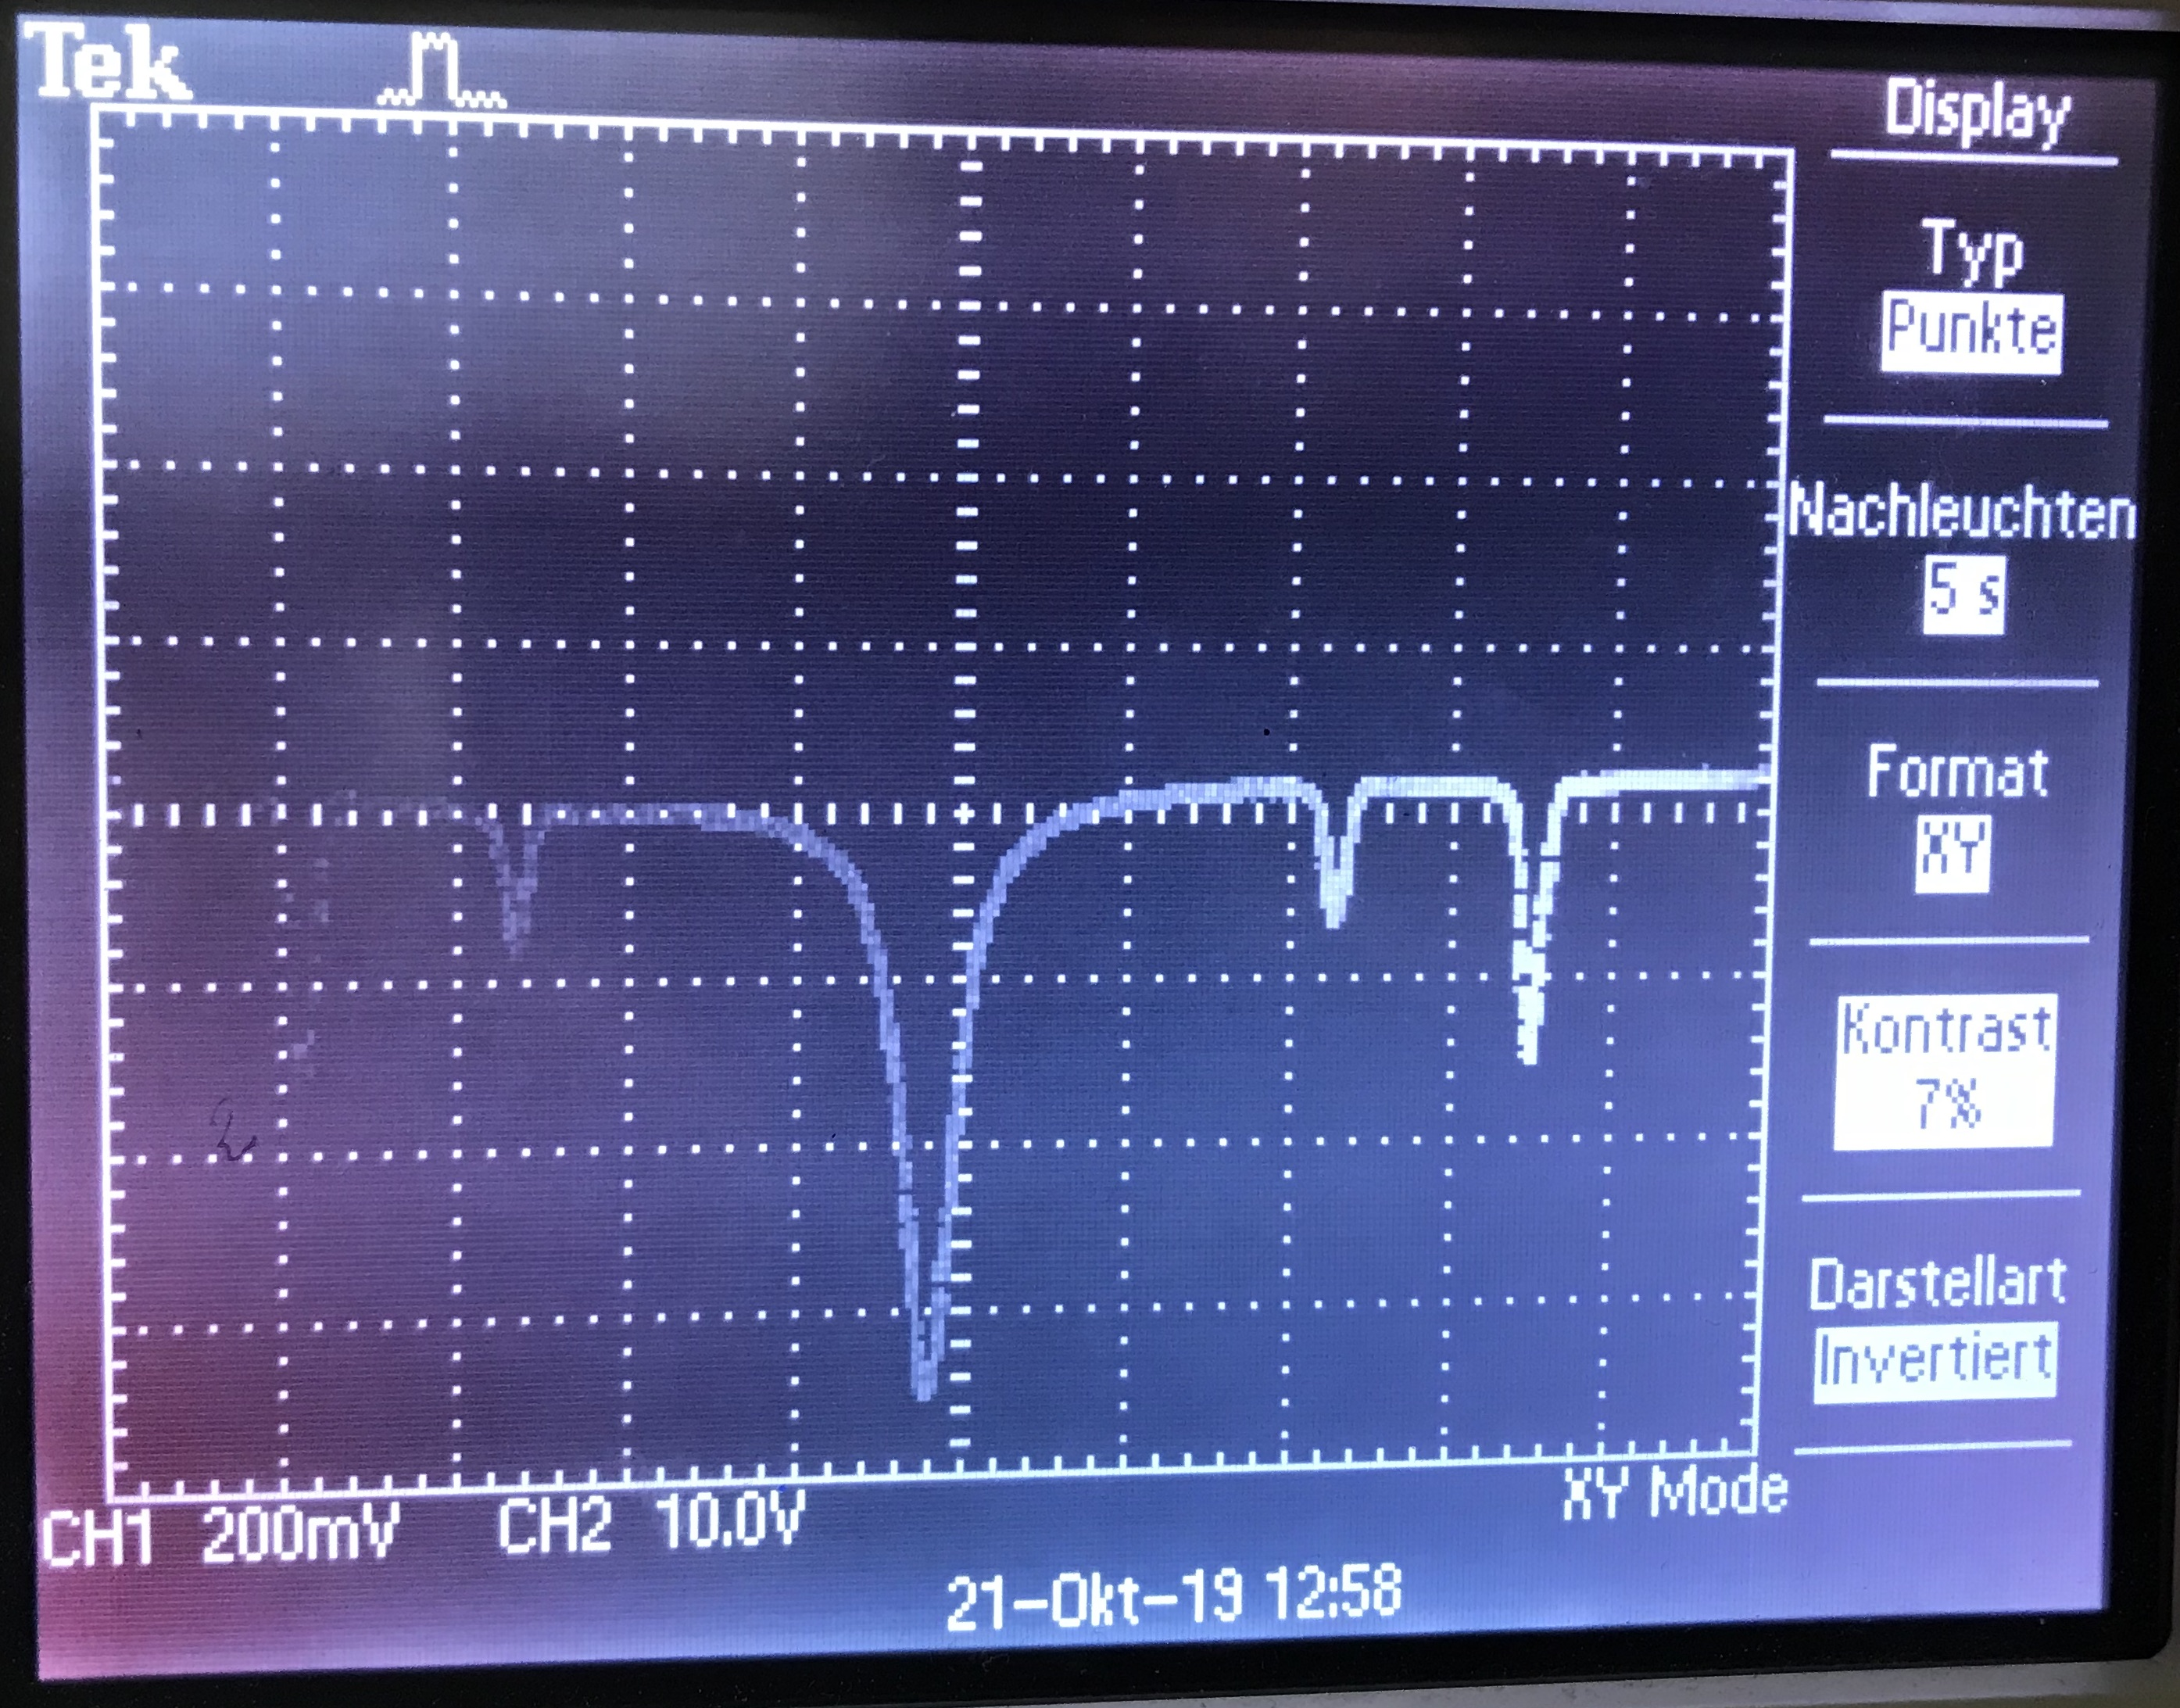
\includegraphics[width=\textwidth]{data/foto.jpg}
  \caption{Typischer Verlauf der Transparenz des Rb-Gases in Abhängigkeit von der magnetischen Feldstärke bei einer Frequenz von $f=100\,$kHz.}
  \label{fig:foto}
\end{figure}

\subsection{Abschätzung des quadratischen Zeeman-Effekts}
\label{subsec:zeeman}
In diesem Kapitel soll abgeschätzt werden, wie groß der Einfluss des quadratischen Zeeman-Effekts
in diesem Versuch ist. Der quadratische Zeeman-Effekt kann beschrieben werden durch Gleichung
\eqref{eqn:zeemanDifferenz}. Gemäß der Versuchsanleitung \cite{Versuchsanleitung} beträgt die
Hyperfeinstrukturaufspaltung des Grundzustandes
\begin{align*}
  \Delta E_{85}&= \SI{2.01e-24}{\joule}\,,\\
  \Delta E_{87}&= \SI{4.53e-24}{\joule}\,.
\end{align*}
Mit den jeweiligen berechneten Werten $B_i$ für die Horizontalkomponente des Erdmagnetfeldes,
$g_{F,i}$ für die Landé-Faktoren und $M_F=1$ ergibt sich damit für den quadratischen Zeeman-Effekt
\begin{align*}
  \Delta E_{Z,85}&= \,,\\
  \Delta E_{Z,87}&= \,.
\end{align*}
Die zusätzlich durch den quadratischen Term herbeigeführte Aufspaltung beträgt dabei lediglich
\begin{align*}
  \Delta E_{quadratisch,85}&= \,,\\
  \Delta E_{quadratisch,87}&= \,.
\end{align*}
Somit ist der quadratische Zeeman-Effekt in diesem Versuch vernachlässigbar.

\subsection{Bestimmung des Verhältnisses der Landé-Faktoren mithilfe der Rabi-Oszillationen}
\label{subsec:oszillationen}
Zur Bestimmung des Verhältnisses der Landé-Faktoren mithilfe der Rabi-Oszillationen werden
die gemessenen Periodendauern der Oszillationen gegen die Amplitude des RF-Feldes aufgetragen.
Die zugehörigen Messwerte befinden sich in Tabelle \ref{tab:oszi}.

\begin{table}[htp]
	\begin{center}
    \caption{Messwerte für die Periodendauern der Oszillationen in Abhängigkeit von der Amplitude des RF-Feldes.}
    \label{tab:oszi}
		\begin{tabular}{ccc}
		\toprule
			{$U$/V} & {$T_1$/ms} & {$T_2$/ms}\\
			\midrule
			2,00 & 1,50 & 2,52\\
			3,00 & 1,16 & 1,84\\
			4,00 & 0,89 & 1,29\\
			5,00 & 0,71 & 1,07\\
			6,00 & 0,61 & 0,90\\
			7,00 & 0,51 & 0,77\\
			8,00 & 0,45 & 0,67\\
			9,00 & 0,40 & 0,60\\
			10,00 & 0,36 & 0,54\\
		\bottomrule
		\end{tabular}
	\end{center}
\end{table}

Außerdem wird eine Ausgleichsrechnung der Form
\begin{equation*}
  f(x)=a+\frac{b}{x-c}
\end{equation*}
durchgeführt. Dies in in den Abbildungen \ref{fig:oszi1} und \ref{fig:oszi2} grafisch dargestellt.
Es ergeben sich die Parameter
\begin{align*}
  a_1&=\SI{}{\second} \,,\\
  b_1&=\SI{}{\volt} \,,\\
  c_1&=\SI{}{\volt} \,,\\
  a_2&=\SI{}{\second} \,,\\
  b_2&=\SI{}{\volt} \,,\\
  c_2&=\SI{}{\volt} \,.
\end{align*}
Das Verhältnis aus $b_1$ und $b_2$ beträgt damit
\begin{equation*}
  \frac{b_1}{b_2}= \,.
\end{equation*}

\begin{figure}
  \centering
  \includegraphics[width=\textwidth]{build/oszi1.pdf}
  \caption{Messwerte und Ausgleichsrechnung zur Bestimmung des Verhältnisses der Landé-Faktoren mithilfe der
  Rabi-Oszillationen für $\text{Rb}^{85}$.}
  \label{fig:oszi1}
\end{figure}
\begin{figure}
  \centering
  \includegraphics[width=\textwidth]{build/oszi2.pdf}
  \caption{Messwerte und Ausgleichsrechnung zur Bestimmung des Verhältnisses der Landé-Faktoren mithilfe der
  Rabi-Oszillationen für $\text{Rb}^{87}$.}
  \label{fig:oszi2}
\end{figure}
